%%%%%%%%%%%%%%%%%%%%%%%%%%%%%%%%%%%%%%%%%
% Beamer Presentation
% LaTeX Template
% Version 1.0 (10/11/12)
%
% This template has been downloaded from:
% http://www.LaTeXTemplates.com
%
% License:
% CC BY-NC-SA 3.0 (http://creativecommons.org/licenses/by-nc-sa/3.0/)
%
%%%%%%%%%%%%%%%%%%%%%%%%%%%%%%%%%%%%%%%%%

%----------------------------------------------------------------------------------------
%	PACKAGES AND THEMES
%----------------------------------------------------------------------------------------

\documentclass{beamer}

\mode<presentation> {

% The Beamer class comes with a number of default slide themes
% which change the colors and layouts of slides. Below this is a list
% of all the themes, uncomment each in turn to see what they look like.

%\usetheme{default}
%\usetheme{AnnArbor}
%\usetheme{Antibes}
%\usetheme{Bergen}
%\usetheme{Berkeley}
%\usetheme{Berlin}
%\usetheme{Boadilla}
%\usetheme{CambridgeUS}
%\usetheme{Copenhagen}
%\usetheme{Darmstadt}
%\usetheme{Dresden}
%\usetheme{Frankfurt}
%\usetheme{Goettingen}
%\usetheme{Hannover}
%\usetheme{Ilmenau}
%\usetheme{JuanLesPins}
%\usetheme{Luebeck}
\usetheme{Madrid}
%\usetheme{Malmoe}
%\usetheme{Marburg}
%\usetheme{Montpellier}
%\usetheme{PaloAlto}
%\usetheme{Pittsburgh}
%\usetheme{Rochester}
%\usetheme{Singapore}
%\usetheme{Szeged}
%\usetheme{Warsaw}

% As well as themes, the Beamer class has a number of color themes
% for any slide theme. Uncomment each of these in turn to see how it
% changes the colors of your current slide theme.

%\usecolortheme{albatross}
%\usecolortheme{beaver}
%\usecolortheme{beetle}
%\usecolortheme{crane}
%\usecolortheme{dolphin}
%\usecolortheme{dove}
%\usecolortheme{fly}
%\usecolortheme{lily}
%\usecolortheme{orchid}
%\usecolortheme{rose}
%\usecolortheme{seagull}
%\usecolortheme{seahorse}
%\usecolortheme{whale}
%\usecolortheme{wolverine}

%\setbeamertemplate{footline} % To remove the footer line in all slides uncomment this line
%\setbeamertemplate{footline}[page number] % To replace the footer line in all slides with a simple slide count uncomment this line

%\setbeamertemplate{navigation symbols}{} % To remove the navigation symbols from the bottom of all slides uncomment this line
}


\usepackage{graphicx} % Allows including images
\usepackage{booktabs} % Allows the use of \toprule, \midrule and \bottomrule in tables
\usepackage{commath} % For norm
\usepackage{multirow}
\usepackage{caption}

%-===========-MY ADDITIONS-======================
%gets rid of bottom navigation bars
\setbeamertemplate{footline}[page number]{}

%gets rid of navigation symbols
\setbeamertemplate{navigation symbols}{}


%----------------------------------------------------------------------------------------
%	TITLE PAGE
%----------------------------------------------------------------------------------------

\title[KM for DL]{Kernel Methods for Deep Learning} % The short title appears at the bottom of every slide, the full title is only on the title page

\author{Akhil P M} % Your name
\institute[] % Your institution as it will appear on the bottom of every slide, may be shorthand to save space
{
Supervisor : Sumitra S \\ % Your institution for the title page
%\medskip
%\textit{john@smith.com} % Your email address
}
\date{\today} % Date, can be changed to a custom date

\begin{document}

\begin{frame}
\titlepage % Print the title page as the first slide
\end{frame}

\begin{frame}
\frametitle{Overview} % Table of contents slide, comment this block out to remove it
\tableofcontents % Throughout your presentation, if you choose to use \section{} and \subsection{} commands, these will automatically be printed on this slide as an overview of your presentation
\end{frame}

%----------------------------------------------------------------------------------------
%	PRESENTATION SLIDES
%----------------------------------------------------------------------------------------

%------------------------------------------------
\section{Review of Arc-cosine Kernel} % Sections can be created in order to organize your presentation into discrete blocks, all sections and subsections are automatically printed in the table of contents as an overview of the talk
%------------------------------------------------
\begin{frame}
\frametitle{Review of Arc-cosine Kernel}
Let x,y be two inputs in $\mathbb{R}^d$. Define $\theta$ as the angle between them given by
\[ \theta = cos^{-1}\left ( \frac{x\cdot y}{\left \| x \right \| \left \| y \right \|} \right ) \]
Then the kernel function computed by the Arc-cosine kernel is
\[ k_n(x,y) = \frac{1}{\pi}\left \| x \right \|^n \left \| y \right \|^n J_n(\theta) \]
where n is called the degree of the kernel and
\[ J_n(\theta) = (-1)^n(sin\theta)^{2n+1} \left ( \frac{1}{sin\theta} \frac{\partial}{\partial \theta} \right )^n \left ( \frac{\pi-\theta}{sin\theta} \right ) \]

\end{frame}

\begin{frame}
\frametitle{Review of Arc-cosine Kernel}
$J_n(\theta)$ for n=0,1,2 is computed as shown below.
\[ J_0(\theta) = \pi-\theta \]
\[ J_1(\theta) = sin\theta + (\pi-\theta)cos\theta \]
\[ J_2(\theta) = 3sin\theta cos\theta + (\pi-\theta)(1+2cos^2\theta) \]
for n=0, it takes the simple form
\[k_0(x,y) =  1- \frac{1}{\pi}cos^{-1}\left ( \frac{x\cdot y}{\left \| x \right \| \left \| y \right \|} \right )  \]
hence the name Arc-cosine kernel is given!
\end{frame}

\begin{frame}
\frametitle{RKHS of Arc-cosine kernel \& Neural Networks}
Consider the single layer neural network shown below with weights $W_{ij}$ connects the $j^{th}$ input unit to the $i^{th}$ output unit. The network maps input $x$ to output $f(x)$ by applying a non-linear map 
\[ f(x) = g(W \cdot x) \]
where the non-linearity is described by the network`s activation function
\[g_n(z) = \Theta(z)z^n \]
with 
\[ \Theta(z) = \frac{1}{2}(1+sign(z)) \]
this activation function is called one-sided polynomial activation function, whose graph for different n values is also shown below.
\end{frame}

\begin{frame}
\frametitle{RKHS of Arc-cosine kernel \& Neural Networks}
\begin{figure}
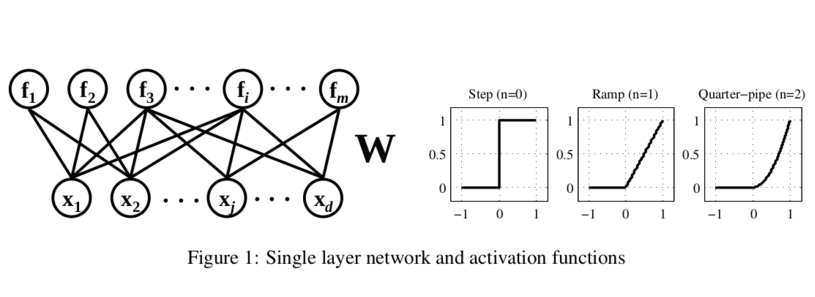
\includegraphics[width=1.0\linewidth, height=7cm]{figures/neuralnet}
\end{figure}
\end{frame}

%\subsection{Subsection Example} % A subsection can be created just before a set of slides with a common theme to further break down your presentation into chunks

\section{Working with Better Features}

\begin{frame}
\frametitle{Autoencoders for Feature Extraction}

\begin{itemize}
\item Feasibility of using an autoencoder for extracting better features is explored.
\item Sparse autoencoder is used in the analysis.
\item Classification accuracy is improved \& the data handling cost is reduced due to the compressed representation of input. 
\end{itemize}
An autoencoder is a neural network trained with backpropagation algorithm (using unsupervised learning) by gradient descent.\\

The aim of an auto-encoder is to learn a compressed, distributed representation (encoding) for a set of data, typically for the purpose of dimensionality reduction.
\end{frame}

\begin{frame}
\frametitle{Feature Compresssion with Autoencoder}
\begin{figure}
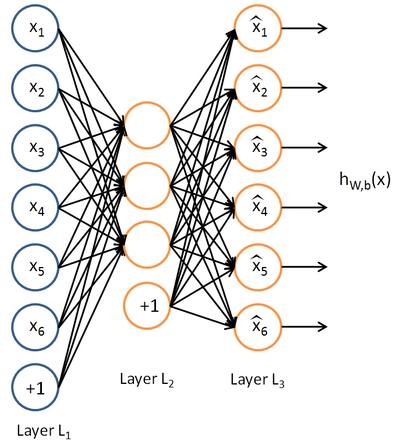
\includegraphics[width=0.7\linewidth, height=7cm]{figures/autoencoder}
\end{figure}
\end{frame}

\begin{frame}
\frametitle{Sparsity Constraint}
\begin{itemize}
\item A coding is said to be \textbf{sparse} when each item is encoded by the strong activation of a relatively small set of neurons.
\item By enforcing sparse coding requirement, we can limit the number of hidden units that can be activated by each input pattern.
\item Given a potentially large set of input patterns, sparse coding algorithms (e.g. Sparse Autoencoder) attempt to automatically find \textit{a small number of representative patterns which, when combined in the right proportions, reproduce the original input patterns}. The sparse coding for the input then consists of those representative patterns.
\item A sparse autoencoder includes a sparseness constraint on hidden layer activation that is enforced by the addition of the Kullback-Leibler (KL) divergence term to the objective function.
\end{itemize}
\end{frame}

\begin{frame}
\frametitle{Sparse Autoencoder}
let $\textstyle{a^{(2)}_j(x)}$ denote the activation of  hidden unit $\textstyle{j}$ when the network is given a specific input $\textstyle{x}$. Further, let 
\[\quad \hat{ \rho_j }= \frac{1}{m} \sum_{i=1}^m \left[ a^{(2)}_j(x^{(i)}) \right] \]
be the average activation of hidden unit $\textstyle{j}$ averaged over the training set. We would like to enforce the constraint
\[ \quad \hat{\rho_j}= \rho \]
where $\textstyle{\rho}$ is a sparsity parameter, typically a small value close to zero(say $\textstyle{\rho = 0.05)}$. To achieve this, we will add an extra penalty term to our optimization objective that penalizes $\textstyle{\hat{\rho_j}}$ deviating significantly from $\textstyle{\rho}$. 
\end{frame}

\begin{frame}
\frametitle{Sparse Autoencoder}
The penalty term is 
\[ \sum_{j=1}^{s_2} {\rm KL}(\rho || \hat\rho_j) = \sum_{j=1}^{s_2} \rho \log \frac{\rho}{\hat\rho_j}
 + (1-\rho) \log \frac{1-\rho}{1-\hat\rho_j} \]
 where $s_2$ is the no of nodes in hidden layer. $\textstyle{{\rm KL}(\rho || \hat\rho_j)=0}$ if $\textstyle{\hat{\rho_j} = \rho}$, otherwise it increases monotonically as $\textstyle{\hat{\rho_j}}$ diverges from $\textstyle{\rho}$. Then the overall cost function now becomes
 \[J_{\rm sparse}(W,b) = J(W,b) + \beta \sum_{j=1}^{s_2} {\rm KL}(\rho || \hat\rho_j)\]
 where $\textstyle{J(W,b)}$ is the usual NN cost function defined as
\[ J(W,b) = \left[ \frac{1}{m} \sum_{i=1}^m J(W,b;x^{(i)},y^{(i)}) \right]
                       + \frac{\lambda}{2} \sum_{l=1}^{n_l-1} \; \sum_{i=1}^{s_l} \; \sum_{j=1}^{s_{l+1}} \left( W^{(l)}_{ji} \right)^2 \]
 
\end{frame}

\begin{frame}
\frametitle{Sparse Autoencoder}
\[= \left[ \frac{1}{m} \sum_{i=1}^m \left( \frac{1}{2} \left\| h_{W,b}(x^{(i)}) - y^{(i)} \right\|^2 \right) \right]
                       + \frac{\lambda}{2} \sum_{l=1}^{n_l-1} \; \sum_{i=1}^{s_l} \; \sum_{j=1}^{s_{l+1}} \left( W^{(l)}_{ji} \right)^2 \]
here $\lambda$ is the regularization parameter.\\
The parameter $\textstyle{\beta}$ controls the weight of the sparsity penalty term.

\end{frame}


\begin{frame}
\frametitle{Performance Comparison}
\begin{figure}
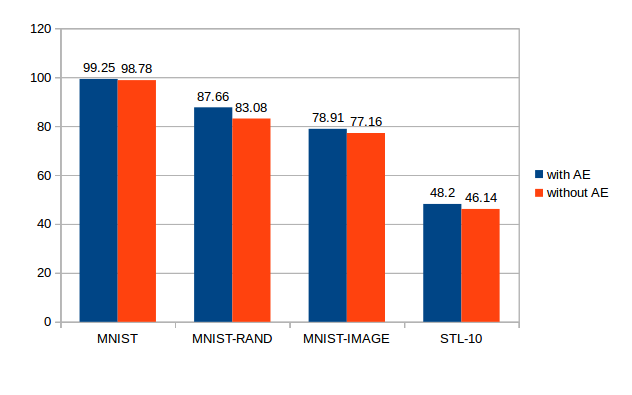
\includegraphics[width=0.8\linewidth, height=7cm]{figures/acc_comparison}
\caption{Accuracy on various datasets with \& without autoencoder}
\end{figure}
\end{frame}

\begin{frame}
\frametitle{Attribute Compression}
\begin{figure}
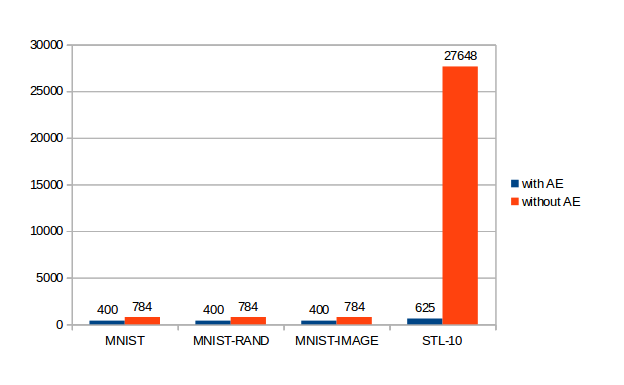
\includegraphics[width=0.8\linewidth, height=7cm]{figures/att_compression}
\caption{Dimensionality reduction obtained with autoencoder}
\end{figure}
\end{frame}
%------------------------------------------------

%------------------------------------------------
\section{Analysis of Decision Boundary}
%------------------------------------------------

\begin{frame}
\frametitle{Analysis of Decision Boundary}
\begin{figure}
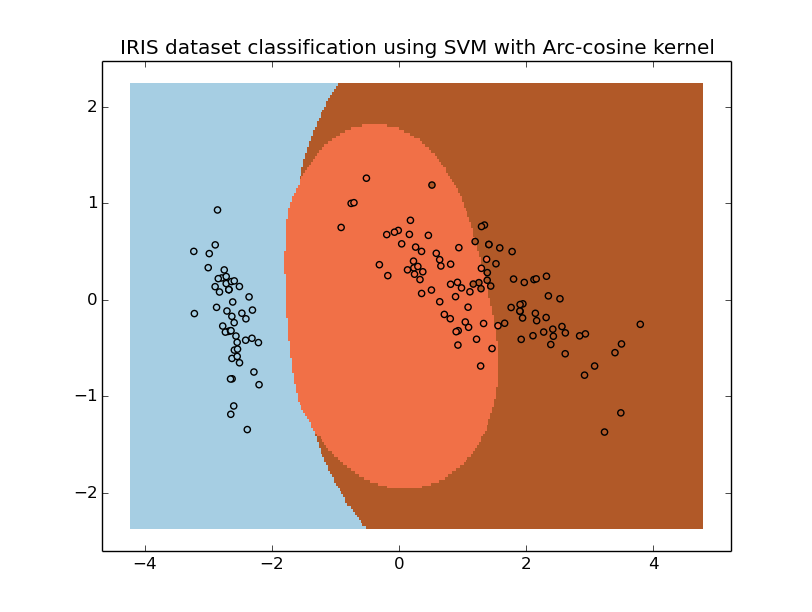
\includegraphics[width=0.7\linewidth, height=6.5cm]{figures/db1_2111}
\caption{when non-linearity is low(kernel parameter = [2,1,1,1])}
\end{figure}
\end{frame}

\begin{frame}
\frametitle{Analysis of Decision Boundary}
\begin{figure}
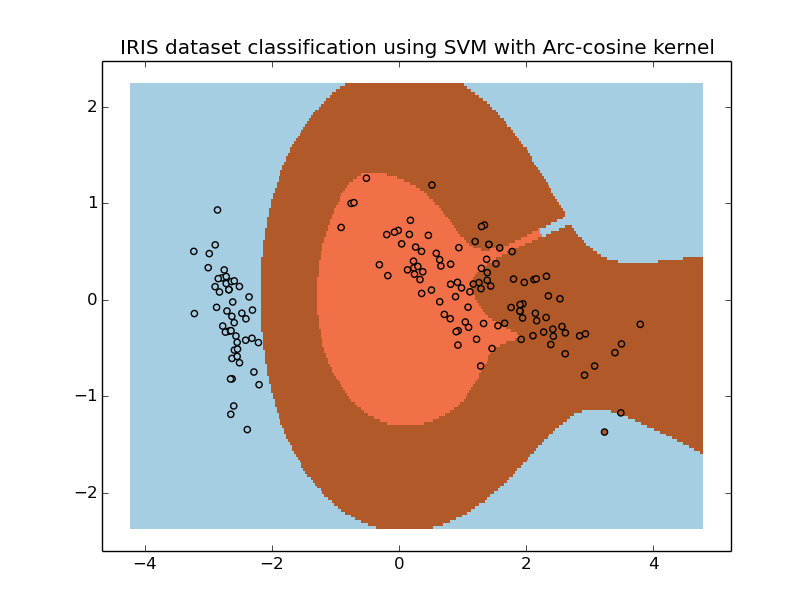
\includegraphics[width=0.7\linewidth, height=6.5cm]{figures/db2_3221}
\caption{when non-linearity is high(kernel parameter = [3,2,2,1])}
\end{figure}
\end{frame}
%------------------------------------------------

%------------------------------------------------
\section{Deep Kernel on Structured Learning Problems}
%------------------------------------------------
\begin{frame}
\frametitle{Deep Kernel on Structured Learning Problems}
Structured output prediction describes the problem of learning a function
\[ h: \mathcal{X} \longrightarrow \mathcal{Y} \]
where $\mathcal{X}$ is the input space and $\mathcal{Y}$ is the output space(structured). To learn $h$, we assume that a training sample of input-output pairs
\[ S = ((x_1, y_1), \ldots, (x_m, y_m)) \in (\mathcal{X} \times \mathcal{Y})^m \]
is available and drawn i.i.d from a distribution P(X,Y).\\
Following empirical risk minimization principle, we will find an $h \in \mathcal{H}$ that minimizes the empirical risk
\[ R_s^{\bigtriangleup} = \frac{1}{m} \sum_{i=1}^m \bigtriangleup(y_i, h(x_i)) \]
\end{frame}


\begin{frame}
\frametitle{StructSVM : Problem Formulation}
Here $\bigtriangleup(y, \overline{y})$ denotes the \textbf{loss} associated with predicting $\overline{y}$ when $y$ is the correct output. Furthermore, we assume that $\bigtriangleup(y,y) = 0 $ and 
\[ \bigtriangleup(y, \overline{y}) \geq 0 \textrm{ for } y \neq \overline{y} \]
\begin{block}{Method}
StructSVM selects an $h \in \mathcal{H}$ that minimizes a regularized empirical risk\\
on $S$. The general idea here is to learn a discriminant function $\mathnormal{f} : \mathcal{X} \times \mathcal{Y} \longrightarrow \mathbb{R}$ over input/output pairs from which one derives a prediction by maximizing $\mathnormal{f}$ over all $y \in \mathcal{Y}$ for a given input $x$
\end{block}
\[ h_w(x) =  \underset{y \in \mathcal{Y}}{\arg\max} \mathnormal{f}_w(x,y) \]
We assume that $\mathnormal{f}_w(x,y)$ takes the form of a linear function
\[ \mathnormal{f}_w(x,y) = \langle w , \Psi(x,y) \rangle \]
\end{frame}

\begin{frame}
\frametitle{StructSVM : Problem Formulation}
where $w \in \mathbb{R}^N$ is a parameter vector and $\Psi(x,y)$ is a combined feature space of relating input $x$ and output $y$.
\begin{block}{Inuitive picture for $\mathnormal{f}_w(x,y)$}
We can think of $\mathnormal{f}_w(x,y)$ as a compatibility function that measures how well the output $y$ matches the given input $x$.
\end{block}
The flexibility in designing $\Psi$ allows us to employ StructSVMs to learn models for problems as diverse as Natural Language Parsing(NLP), Protein Sequence Alignment, Image Segmentation etc.\\
Joachims et.al proposed two different ways of using a hinge loss to convex upper bound the loss.\\
1. \textbf{Margin Rescaling}(MR)\\
In MR the position of the hinge is adapted keeping the slope fixed. 
\end{frame}

\begin{frame}
\frametitle{StructSVM : Problem Formulation}
\[ \bigtriangleup_{MR}(y, h_w(x)) =  \underset{y \in \mathcal{Y}}{\max}\{ \bigtriangleup(y, \overline{y}) - \langle w , \Psi(x,y) \rangle + \langle w , \Psi(x,\overline{y}) \rangle \} \]
\[ \geq \bigtriangleup(y, h_w(x)) \]
1. \textbf{Slack Rescaling}(SR)\\
In SR the slope is adjusted while keeping the position of the hinge fixed.
\[ \bigtriangleup_{SR}(y, h_w(x)) =  \underset{y \in \mathcal{Y}}{\max}\{ \bigtriangleup(y, \overline{y})(1 - \langle w , \Psi(x,y) \rangle + \langle w , \Psi(x,\overline{y}) \rangle) \} \]
\[ \geq \bigtriangleup(y, h_w(x)) \]
This leads to the following optimization problems, where each slack variable $\xi_i$ is equal to the respective $\bigtriangleup_{MR}(y_i, h_w(x_i))$ or $\bigtriangleup_{SR}(y_i, h_w(x_i))$ for the training example $(x_i, y_i)$.
\end{frame}


\begin{frame}
\frametitle{StructSVM : Problem Formulation}
\begin{block}{n-Slack StructSVM with Margin Rescaling}
\[\underset{w, \xi \geq 0}{\min} \quad \frac{1}{2} \norm{w}^2 + \frac{C}{n} \sum_{i=1}^m \xi_i \]
\[ \textrm{s.t } \forall \overline{y_1} \in \mathcal{Y} \textrm{  :  } w^T[\Psi(x_1, y_1) - \Psi(x_1, \overline{y_1})] \geq \bigtriangleup(y_1, \overline{y_1}) - \xi_1 \]
\[ \vdots \]
\[ \textrm{s.t } \forall \overline{y_m} \in \mathcal{Y} \textrm{  :  } w^T[\Psi(x_m, y_m) - \Psi(x_m, \overline{y_m})] \geq \bigtriangleup(y_m, \overline{y_m}) - \xi_m \]
\end{block}

\end{frame}

\begin{frame}
\frametitle{StructSVM : Problem Formulation}
\begin{block}{n-Slack StructSVM with Slack Rescaling}
\[\underset{w, \xi \geq 0}{\min} \quad \frac{1}{2} \norm{w}^2 + \frac{C}{n} \sum_{i=1}^m \xi_i \]
\[ \textrm{s.t } \forall \overline{y_1} \in \mathcal{Y} \textrm{  :  } w^T[\Psi(x_1, y_1) - \Psi(x_1, \overline{y_1})] \geq 1 - \frac{\xi_1}{\bigtriangleup(y_1, \overline{y_1})} \]
\[ \vdots \]
\[ \textrm{s.t } \forall \overline{y_m} \in \mathcal{Y} \textrm{  :  } w^T[\Psi(x_m, y_m) - \Psi(x_m, \overline{y_m})] \geq 1 - \frac{\xi_m}{\bigtriangleup(y_m, \overline{y_m})} \]
\end{block}
The constraints states that for each training example, $(x_i, y_i)$ the score $w^T[\Psi(x_i, y_i)$ must be greater than the score $w^T[\Psi(x_i, \overline{y})$ of all outputs $\overline{y} \in \mathcal{Y}$ by a required margin. This margin is 1 in SR and $\bigtriangleup(y, \overline{y})$ in MR.
\end{frame}


\begin{frame}
\frametitle{StructSVM : Challenges}
\begin{itemize}
\item This optimization problem has $\mathcal{O}(m|\mathcal{Y}|)$ \textbf{number of constraints}, where $|\mathcal{Y}|$ is typically extremely large(usually exponential to the description length of y). This makes standard QP solvers unsuitable for this type of problem.

\item Thus for solving the optimizaion problem \textbf{cutting plane algorithm} is used. It will utilize the special structure of the max-margin problem, so that only a much smaller subset of constraints need to be explicitly examined.

\item The cutting plane algorithm iteratively generates cutting planes over a convex set, effectively shrinking the size of the set at a faster rate so that the optimum solution will be reached very fast.

\item The convex function that we will minimize over this convex set is our objective function.
\end{itemize}

\end{frame}


\begin{frame}
\frametitle{StructSVM : Experimental Results on Small Datasets}
\begin{table}[htb]
\centering
\captionsetup{justification=centering}
\begin{tabular}{| l | l | l |}
\toprule
\textbf{Dataset} & \textbf{Arc-Cosine Kernel} & \textbf{Other Kernel(best)}\\
\midrule
Scene Segentation & 69.65\% & 69.4\% \\
(multilabel - 6 class) & & \\
\hline
Vehicle Dataset & 73.52\% & 75.1\% \\
(multiclass - 4 class) & & \\
\hline
Iris Dataset & 98.33\% & 96.67\% \\
(multiclass - 3 class) & & \\
\hline
Breast Cancer Wiscosin & 99.02\% & 99.02\% \\
(binary) & & \\
\hline
Synthetic Data & 66.15\% & 67.45\% \\
(multiclass - 7 class) & & \\
\bottomrule
\end{tabular}
\caption{Performance comparison of Arc-cosine kernel to other kernels on small datasets in StructSVM framework}
\end{table}
\end{frame}


\section{Future Plans}

\begin{frame}
\frametitle{Future Plans}
\begin{itemize}
\item Explore the scope of deep kernels on structured learning problems.

\item Build a scalable version of structSVM for large datasets.

\item Enhance the learning process by using Active Learning techniques.

\item Try more techniques for feature engineering like Convolutional Neural Networks, Stacked Autoencoders etc.
\end{itemize}

\end{frame}

\begin{frame}
\frametitle{References}
\footnotesize{
\begin{thebibliography}{99} % Beamer does not support BibTeX so references must be inserted manually as below
\bibitem[Saul, 2009]{p1} Y. Cho, L.K. Saul, Kernel Methods  for Deep Learning
\newblock \emph{Advances in Neural Information Processing Systems(NIPS) 22}, 342 -- 350, 2009.

\bibitem[Tsochantaridis, 2005]{p1} I. Tsochantaridis, T. Joachims, T. Hoffman, Y. Altun, Large Margin Methods for Structured and Interdependent Output SPaces
\newblock \emph{Journel of Machine Learning Research(JMLR) 6}, 1453 -- 1484, 2005.

\bibitem[Joachims, 2009]{p1} T. Joachims, T. Finely, C. John Nu, Cutting-Plane Training on Structural SVMs
\newblock \emph{Journal of Machine Learning 77(1)}, 27 -- 59, 2009.

\bibitem[Kelley, 1960]{p1} J.E Kelley, The Cutting-plane Method for Solving Convex Programs
\newblock \emph{Journel of the Society for Industrial and Applied Mathematics(SIAM) 8}, 703 -- 712, 1960.

\bibitem[Koller, 2000]{p1} S. Tong, D. Koller, Support Vector Machine Active Learning with Applications to Text Classification
\newblock \emph{In Proceedings of the $7^{th}$ International Conference on Machine Learning(ICML)}, 287 -- 295, 2000.


\end{thebibliography}
}
\end{frame}

\iffalse
%commented region

\begin{frame}
\frametitle{Multiple Columns}
\begin{columns}[c] % The "c" option specifies centered vertical alignment while the "t" option is used for top vertical alignment

\column{.45\textwidth} % Left column and width
\textbf{Heading}
\begin{enumerate}
\item Statement
\item Explanation
\item Example
\end{enumerate}

\column{.5\textwidth} % Right column and width
Lorem ipsum dolor sit amet, consectetur adipiscing elit. Integer lectus nisl, ultricies in feugiat rutrum, porttitor sit amet augue. Aliquam ut tortor mauris. Sed volutpat ante purus, quis accumsan dolor.

\end{columns}
\end{frame}

%------------------------------------------------
\section{Second Section}
%------------------------------------------------

\begin{frame}
\frametitle{Table}
\begin{table}
\begin{tabular}{l l l}
\toprule
\textbf{Treatments} & \textbf{Response 1} & \textbf{Response 2}\\
\midrule
Treatment 1 & 0.0003262 & 0.562 \\
Treatment 2 & 0.0015681 & 0.910 \\
Treatment 3 & 0.0009271 & 0.296 \\
\bottomrule
\end{tabular}
\caption{Table caption}
\end{table}
\end{frame}

%------------------------------------------------

\begin{frame}
\frametitle{Theorem}
\begin{theorem}[Mass--energy equivalence]
$E = mc^2$
\end{theorem}
\end{frame}

%------------------------------------------------

\begin{frame}[fragile] % Need to use the fragile option when verbatim is used in the slide
\frametitle{Verbatim}
\begin{example}[Theorem Slide Code]
\begin{verbatim}
\begin{frame}
\frametitle{Theorem}
\begin{theorem}[Mass--energy equivalence]
$E = mc^2$
\end{theorem}
\end{frame}\end{verbatim}
\end{example}
\end{frame}

%------------------------------------------------


%------------------------------------------------

\begin{frame}[fragile] % Need to use the fragile option when verbatim is used in the slide
\frametitle{Citation}
An example of the \verb|\cite| command to cite within the presentation:\\~

This statement requires citation \cite{p1}.
\end{frame}

%------------------------------------------------

\fi

%------------------------------------------------

\begin{frame}
%\Huge{\centerline{The End}}
\begin{figure}

\includegraphics[width=0.7\linewidth, height=7.5cm]{figures/thankyou}
\end{figure}
\end{frame}

%----------------------------------------------------------------------------------------

\end{document} 